\section{Cel dokumentu}
\suppressfloats[t]

Niniejszy dokument powstał w celu przedstawienia wszystkich poziomów uprawnień które znajdą się w Systemie Obsługi Konferencji (SOK), oraz akcji (przypadków użycia) jakie użytkownik o danym zakresie uprawnień może wykonać w systemie. 

\section{Dokumentyi pliki powiązane}

\begin{itemize}
  \item \textit{administrator.vsdx} - dokument przypadków użycia użytkownika ADMINISTRATOR (plik programu Microsoft Visio 2013)
  \item \textit{administrator.jpg} - wyeksportowany dokument przypadków użycia użytkownika ADMINISTRATOR
  \item \textit{pracownik.vsdx} - dokument przypadków użycia użytkownika PRACOWNIK (plik programu Microsoft Visio 2013)
  \item \textit{pracownik.jpg} - wyeksportowany dokument przypadków użycia użytkownika PRACOWNIK
  \item \textit{rodzina.vsdx} - dokument przypadków użycia użytkownika RODZINA PRACOWNIKA (plik programu Microsoft Visio 2013)
  \item \textit{rodzina.jpg} - wyeksportowany dokument przypadków użycia użytkownika RODZINA PRACOWNIKA 
\end{itemize}

\section{Poziomy uprawnień}

W systemie, zgodnie z wstępnymi ustaleniami, zostaną zaimplementowane 3 poziomy uprawnień. \newline
Pierwszą grupę (najprawdopodobniej jednoosobową) stanowili będą użytkownicy o poziomie uprawnień ADMINISTRATOR SYSTEMU, jest to grupa o prawach nadrzędnych, będzie widziała co się dzieje w całym systemie. Do członków tej grupy należało będzie tworzenie konferencji, zarządzanie nią, dodawanie kont pracowników i inne akcje, o czym później. \newline
Druga grupa to użytkownicy o poziomie uprawnień PRACOWNIK, pracownik otrzyma swoje konto od administratora systemu po utrzednim zgłoszeniu takiej chęci. Pracownik będzie mógł dodawać konto swojej rodzinie, dodać temat do dyskusji do kalendarza konferencji itd. \newline
Ostatnia, trzecia grupa to RODZINA PRACOWNIKA, jak sama nazwa wskazuje będzie to konto które będzie przysługiwało kilku osobom i tu krótkie wyjaśnienie. Pracownik najczęściej do konta rodzinnego doda żonę lub męża i ewentualnie dzieci które w większości nie będą najprawdopodobniej umiały posługiwać się systemem z powodu swojego młodzięczego wieku, dlatego do konta rodzina pracownika będzie można przypisać więcej niż jedną osobę, oczywiście pracownik będzie mógł dodać kilka kont typu rodzina pracownika, co może być przydatne jeżeli na przykład poza żoną i dziećmi będzie chciał zaprosić kolegę, lub siostrę na wyjazd. Czyli podsumowując, do jednego konta typu rodzina pracownika będzie można dodać kilka fizycznych osób. Konto to będzie miało dostęp tylko do części krajoznawczo turystycznej, innych nie będzie widział.

\section{Przypadki użycia}

Słowo wyjaśnienia, przypadki użycia to technika stosowana w inżynierii oprogramowania w celu opisania wymagań tworzonego systemu informatycznego. Przypadek użycia przedstawia interakcję pomiędzy aktorem (użytkownikiem systemu), który inicjuje zdarzenie oraz samym systemem.\newline
Poniżej zostaną przedstawione wstępnie przygotowane diagramy przypadków użycia użytkowników o konkretnych uprawnieniach.

\subsection{Administrator Systemu}

\begin{figure}[!tb]
    \centering
    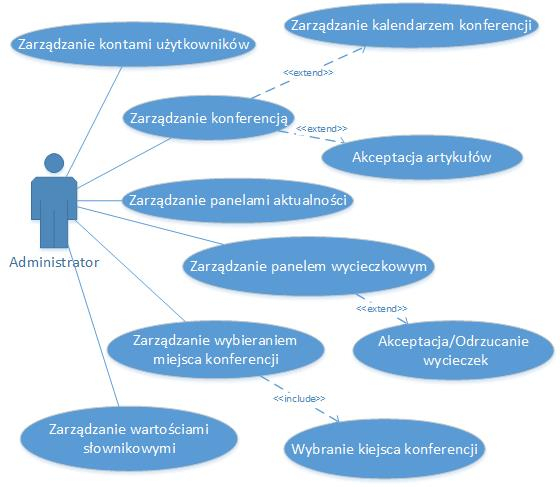
\includegraphics{administrator.jpg}
    \caption{Model diagramu przypadków użycia użytkownika administrator.}
    \label{fig:administrator}
\end{figure}

Administrator będzie pełnił rolę nadzorczą nad całym systemem. Po zalogowaniu do konta zostanie przeniesiony do panelu startowego z którego będzie mógł dodać konferencję i/lub wybrać istniejącą konferencję z listy rozwijanej. Wtedy zostanie przeniesiony do panelu aktualności wybranej konferencji, w którym będzie miał możliwość edycji i publikacji treści. \newline
Stąd będzie mógł się udać na przykład do panelu zarządzania gdzie będzie mógł przydzielać konta pracownikom. zmieniać swoje dane teleadresowe i tym podobne. \newline
Administrator będzie zarządzał również wartościami słownikowymi systemu, czyli na przykład słownikiem możliwych specjalizacji pracowników, który to słownik będzie służył algorytmowi doboru recenzenta do artykułu. \newline
W panelu wycieczek administrator będzie mógł akceptować/odrzucać pomysły wycieczek dodawanych przez innych użytkowników, będzie mógł też dodać swoje propozycje. jakiś czas przed rozpoczęciem konferencji administrator będzie musiał zadecydować które wycieczki się odbędą, a które nie (na przykład z powodu małej ilości chętnych). \newline
Administrator będzie zarządzał również przebiegiem samej konferencji. Po pierwsze do niego będą wpadały tematy artykułów proponowane przez pracowników w celu ich akceptacji. Po drugie administrator będzie zarządzał kalendarzem konferencji tj. będzie planował na osi czasu wystąpienia poszczególnych prelegentów i ustalał agendę konferencji.


\subsection{Pracownik}

\begin{figure}[!tb]
    \centering
    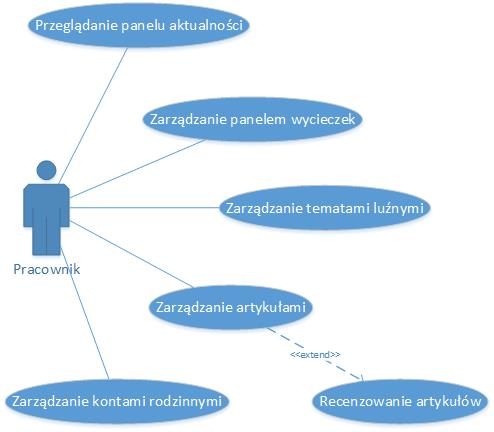
\includegraphics{pracownik.jpg}
    \caption{Model diagramu przypadków użycia użytkownika pracownik.}
    \label{fig:pracownik}
\end{figure}

Pracownik będzie miał dostęp do wszystkich paneli w systemie. Po zalogowaniu do systemu wybierze z listy rozwijanej konferencję i zostanie przeniesiony do panelu aktualności, którego będzie miał możliwość podglądu. Stąd będzie mógł przejść do ustawień swojego konta gdzie będzie mógł między innymi dodać konto rodziny oraz zmienić swoje dane teleadresowe.  \newline
Pracownik będzie miał możliwość dodania propozycji wycieczki która trafi do akceptacji przez administratora, będzie również mógł zgłosić chęć udziału w wycieczkach zaproponowanych przez innych użytkowników. \newline
W panelu tematów luźnych będzie mógł dodać propozycję swojego tematu która trafi do akceptacji przez administratora, wiąże się to z tym że w szczególności przez dwóch pracowników może zostać zaproponowany podobny temat, wtedy administrator będzie mógł wstawić je do kalendarza w tym samym miejscu, albo jeden po drugim. \newline
Najbardziej rozbudowaną funkcjonalnością pracownika będzie panel zarządzania artykułami, tutaj pracowniik będzie zgłaszał temat swojego arytkułu, następnie pisał go przy użyciu odpowiedniego szablonu, później artykuł trafi do recenzenta. Recenzentami arytkułów będą sami pracownicy, system będzie przydzielał do każdego artykułu recenzenta przy użyciu odpowiedniego algorytmu.


\subsection{Rodzina pracownika}

\begin{figure}[!tb]
    \centering
    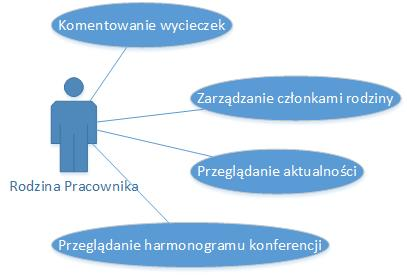
\includegraphics{rodzina.jpg}
    \caption{Model diagramu przypadków użycia użytkownika rodzina pracownika.}
    \label{fig:rodzina}
\end{figure}

Użytkownik konta rodzina pracownika będzie miał dostęp jedynie do modułu wycieczkowego oraz podgląd panelu aktualności. Po zalogowaniu wybierze z listy rozwijanej konferencję i zostanie przeniesiony do panelu aktualności, którego to będzie miał jedynie podgląd. Z panelu aktualności użytkownik może przejść do ustawień swojego konta, gdzie może zarządzać członkami swojej rodziny oraz zmieniać na przykład swoje dane kontaktowe. \newline
Najciekawszym panelem dla rodziny pracownika będzie moduł wycieczkowy, użytkownik będzie miał możliwość zgłoszenia pomysłu swojej wycieczki, pomysł taki trafi do administratora w celu akceptacji przed pojawieniem się w panelu. Użytkownik będzie miał również możliwość zgłoszenia chęci udziału w propozycjach innych wycieczek.

\section{Historia Zmian}

\begin{tabularx}{\textwidth}{X|l|X}
\hline
\textbf{Data zmiany} & \textbf{Kto zmienił} & \textbf{Co zostało zmienione} \\ \hline
11 mar 2015          & Błądek Piotr         & Utworzenie dokumentu          \\ \hline
11 mar 2015          &Błądek Piotr          &  Dodanie historii zmian            \\ \hline
13 mar 2015          &Błądek Piotr          &  Dodanie dokumentów powiązanych i przypadków użycia            \\ \hline
13 mar 2015          &Błądek Piotr          &  Dodanie spisu rysunków            \\ \hline
\end{tabularx}